\documentclass[11pt]{article}
\usepackage[margin=1in]{geometry}
\usepackage{amsmath,amssymb,amsthm,mathtools}
\usepackage{mathrsfs}
\usepackage{tikz}
\usetikzlibrary{arrows.meta,calc,intersections,decorations.markings}

\title{Why We Fix a Lattice with $\Im(\omega_2/\omega_1)>0$}
\author{}
\date{}

\theoremstyle{definition}
\newtheorem{definition}{Definition}
\newtheorem{remark}{Remark}
\theoremstyle{plain}
\newtheorem{proposition}{Proposition}
\newtheorem{theorem}{Theorem}
\newtheorem{lemma}{Lemma}

\newcommand{\C}{\mathbb{C}}
\newcommand{\R}{\mathbb{R}}
\newcommand{\Z}{\mathbb{Z}}
\newcommand{\Hh}{\mathfrak{H}} % upper half-plane

\begin{document}
	\maketitle
	
	\section*{0. Goal}
	We explain, in full detail, the standard normalization
	\[
	\Lambda=\Z\omega_1+\Z\omega_2\subset\C,\qquad \Im\!\left(\frac{\omega_2}{\omega_1}\right)>0,
	\]
	used when defining a complex torus \(X=\C/\Lambda\). This single inequality enforces:
	\begin{itemize}
		\item \emph{Nondegeneracy:} \(\omega_1,\omega_2\) are \(\R\)-linearly independent.
		\item \emph{Orientation:} the ordered basis \((\omega_1,\omega_2)\) has positive signed area.
		\item \emph{Normalization / moduli:} every torus is represented by a unique parameter \(\tau=\omega_2/\omega_1\) \emph{in the upper half-plane} \(\Hh=\{\tau\in\C:\Im\tau>0\}\) up to the natural \(\mathrm{SL}_2(\Z)\)-symmetry.
	\end{itemize}
	
	\section*{1. Lattices and nondegeneracy}
	\begin{definition}[Lattice in \(\C\)]
		A \emph{lattice} is a discrete, rank-2 additive subgroup \(\Lambda\subset\C\), i.e.
		\[
		\Lambda=\Z\omega_1+\Z\omega_2
		\]
		with \(\omega_1,\omega_2\in\C\) that are linearly independent over \(\R\).
	\end{definition}
	
	\begin{proposition}[Nondegeneracy via the ratio]\label{prop:nondeg}
		Let \(\omega_1,\omega_2\in\C\setminus\{0\}\). Then \(\omega_1,\omega_2\) are \(\R\)-linearly independent (i.e. span a rank-2 lattice) if and only if
		\[
		\tau:=\frac{\omega_2}{\omega_1}\notin\R \iff \Im(\tau)\neq 0.
		\]
	\end{proposition}
	
	\begin{proof}
		Write \(\omega_j=a_j+ib_j\) with \(a_j,b_j\in\R\). R-linear dependence means \(\omega_2=t\,\omega_1\) for some \(t\in\R\), equivalently \(\tau\in\R\). If \(\tau\notin\R\), then writing
		\[
		\omega_1=\begin{pmatrix}a_1\\ b_1\end{pmatrix},\quad
		\omega_2=\begin{pmatrix}a_2\\ b_2\end{pmatrix}\in\R^2,
		\]
		the matrix \(M=[\,\omega_1\,\ \omega_2\,]=\begin{psmallmatrix} a_1 & a_2 \\ b_1 & b_2\end{psmallmatrix}\) has nonzero determinant (see Lemma~\ref{lem:area} below), hence the vectors are independent.
	\end{proof}
	
	\section*{2. Orientation and the signed area}
	Given ordered vectors \(\omega_1,\omega_2\in\C\cong\R^2\), the \emph{signed area} of the fundamental parallelogram
	\[
	P=\{ s\,\omega_1+t\,\omega_2 : s,t\in[0,1]\}
	\]
	is the determinant
	\[
	\mathrm{Area}_{\pm}(\omega_1,\omega_2)=\det
	\begin{pmatrix}
		\Re\omega_1 & \Re\omega_2\\[2pt]
		\Im\omega_1 & \Im\omega_2
	\end{pmatrix}.
	\]
	Its absolute value is the geometric area; its sign records orientation.
	
	\begin{lemma}[Determinant identity]\label{lem:area}
		For \(\omega_1\neq 0\) and \(\tau=\omega_2/\omega_1\),
		\[
		\mathrm{Area}_{\pm}(\omega_1,\omega_2)
		=|\omega_1|^2\,\Im(\tau).
		\]
		In particular, \(\mathrm{sign}\big(\mathrm{Area}_{\pm}\big)=\mathrm{sign}\big(\Im(\tau)\big)\).
	\end{lemma}
	
	\begin{proof}
		Write \(\omega_1=r e^{i\theta}\) with \(r>0\). Then
		\[
		\omega_2=\tau\omega_1=r e^{i\theta}\tau.
		\]
		Rotating by \(e^{-i\theta}\) (an area-preserving real linear isomorphism) sends the pair \((\omega_1,\omega_2)\) to \((r,\,r\tau)\). The determinant scales by \(r^2\) and becomes
		\[
		\det\begin{pmatrix} r & r\Re\tau\\ 0 & r\Im\tau\end{pmatrix}
		=r^2\,\Im\tau
		=|\omega_1|^2\,\Im(\tau).
		\]
	\end{proof}
	
	\begin{proposition}[Orientation normalization]
		Replacing \((\omega_1,\omega_2)\) by \((\omega_2,\omega_1)\) sends \(\tau\mapsto 1/\tau\), which flips the sign of \(\Im(\tau)\). Thus, by swapping the two generators if needed, we may assume
		\[
		\Im(\omega_2/\omega_1)>0,
		\]
		i.e. the ordered basis has positive orientation and positive signed area.
	\end{proposition}
	
	\begin{remark}[What if \(\Im(\tau)=0\)?]
		Then \(\tau\in\R\) and Lemma~\ref{lem:area} gives zero area; the two vectors lie on one real line, so \(\Z\omega_1+\Z\omega_2\) is rank~1, not a lattice in the sense we need.
	\end{remark}
	
	\section*{3. Scaling and the single complex parameter \(\tau\)}
	\begin{proposition}[Scaling does not change the torus up to isomorphism]
		For any \(\lambda\in\C^\times\), the map \(z\mapsto \lambda z\) induces a biholomorphism
		\[
		\C/\Lambda \;\xrightarrow{\ \cong\ }\; \C/(\lambda\Lambda),\qquad \Lambda=\Z\omega_1+\Z\omega_2.
		\]
	\end{proposition}
	
	\begin{proof}
		The map is \(\C\to\C\), holomorphic, surjective, and \(\lambda\Lambda\)-periodic; its kernel is exactly \(\Lambda\). Hence it descends to a holomorphic bijection with holomorphic inverse \(z\mapsto \lambda^{-1}z\).
	\end{proof}
	
	\noindent
	\textbf{Normalization by scaling.} Taking \(\lambda=\omega_1^{-1}\) we may assume \(\omega_1=1\). Then the lattice is
	\[
	\Lambda=\Z+\Z\tau,\qquad \tau=\omega_2/\omega_1.
	\]
	By the orientation choice above, we further assume \(\tau\in\Hh=\{\Im\tau>0\}\).
	
	\section*{4. Change of basis and the \(\mathrm{SL}_2(\Z)\)-action}
	Different \emph{bases} can generate the \emph{same} lattice.
	
	\begin{proposition}[Same lattice, new basis]
		Let \(\begin{psmallmatrix} a&b\\ c&d\end{psmallmatrix}\in\mathrm{SL}_2(\Z)\).
		Then
		\[
		(\omega_1',\omega_2')=(a\omega_1+b\omega_2,\; c\omega_1+d\omega_2)
		\]
		is a new ordered \(\Z\)-basis of the same lattice \(\Lambda\).
	\end{proposition}
	
	\begin{proof}
		The matrix is unimodular, so the change of basis is invertible over \(\Z\), and
		\(
		\Z\omega_1'+\Z\omega_2'=\Z\omega_1+\Z\omega_2.
		\)
	\end{proof}
	
	\begin{proposition}[Möbius action on \(\tau\)]
		If \(\tau=\omega_2/\omega_1\) and \((\omega_1',\omega_2')=(a\omega_1+b\omega_2,\ c\omega_1+d\omega_2)\) with \(\begin{psmallmatrix}a&b\\ c&d\end{psmallmatrix}\in\mathrm{SL}_2(\Z)\), then
		\[
		\tau'=\frac{\omega_2'}{\omega_1'}=\frac{c\omega_1+d\omega_2}{a\omega_1+b\omega_2}
		=\frac{c+d\tau}{a+b\tau}.
		\]
		Equivalently, writing the basis as \((1,\tau)\), the action on \(\tau\) is the Möbius map
		\[
		\tau\longmapsto \frac{a\tau+b}{c\tau+d}.
		\]
	\end{proposition}
	
	\begin{proof}
		Factor out \(\omega_1\neq 0\) to reduce to the pair \((1,\tau)\) and compute directly.
	\end{proof}
	
	\begin{lemma}[Upper half-plane is preserved]
		For \(\begin{psmallmatrix}a&b\\ c&d\end{psmallmatrix}\in\mathrm{SL}_2(\Z)\) and \(\tau\in\Hh\),
		\[
		\Im\!\left(\frac{a\tau+b}{c\tau+d}\right)=\frac{\Im(\tau)}{|c\tau+d|^2}>0.
		\]
	\end{lemma}
	
	\begin{proof}
		Compute
		\(
		\frac{a\tau+b}{c\tau+d}
		=\frac{(a\tau+b)(\overline{c\tau+d})}{|c\tau+d|^2}
		\)
		and take imaginary parts. The numerator simplifies to \(\Im(\tau)\) using \(ad-bc=1\).
	\end{proof}
	
	\noindent
	\textbf{Conclusion.} Two bases related by \(\mathrm{SL}_2(\Z)\) define the same lattice; they differ by the Möbius action on \(\tau\), which preserves \(\Hh\). Thus the \emph{moduli} of complex tori is the quotient
	\[
	\mathrm{Tori}(\C)\ \cong\ \mathrm{SL}_2(\Z)\backslash \Hh,
	\]
	and the condition \(\Im(\omega_2/\omega_1)>0\) is exactly “choose the representative \(\tau\) in the upper half-plane.”
	
	\section*{5. Putting it together (one line)}
	After scaling so that \(\omega_1=1\) and choosing the ordered basis to make the signed area positive, we \emph{fix}
	\[
	\Lambda=\Z+\Z\tau \quad\text{with}\quad \tau\in\Hh\ \ (\Im\tau>0).
	\]
	This simultaneously encodes nondegeneracy, orientation, and normalization modulo the \(\mathrm{SL}_2(\Z)\)-symmetry.
	
	\section*{6. Figures}
	
	\subsection*{Figure A: Orientation and signed area}
	\begin{center}
		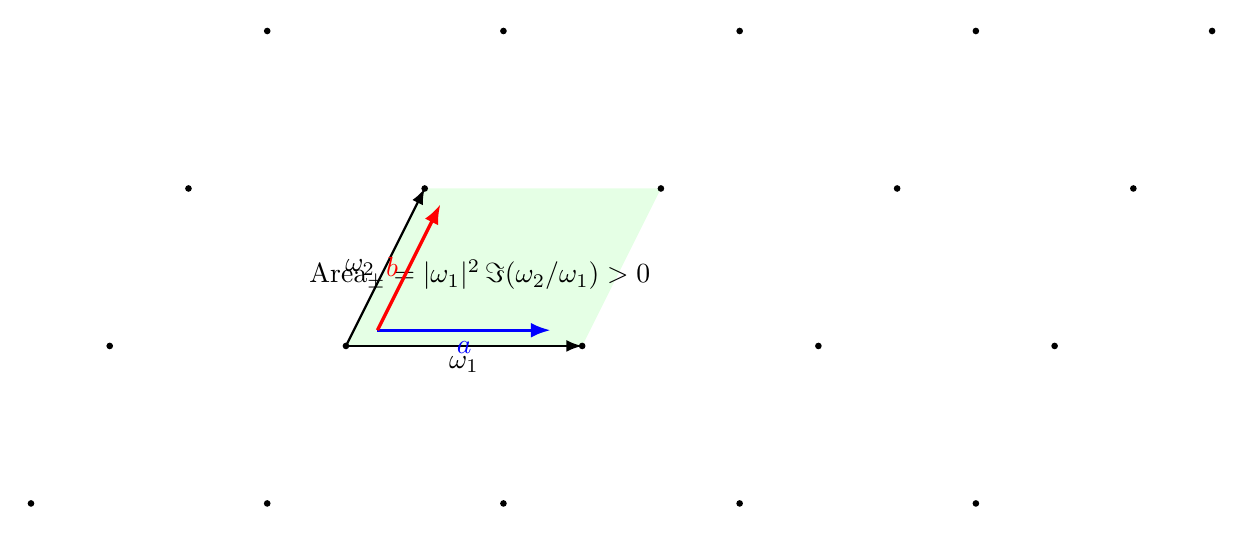
\begin{tikzpicture}[scale=1.0]
			\coordinate (O) at (0,0);
			\coordinate (w1) at (3,0);       % omega_1 real
			\coordinate (w2) at (1,2);       % omega_2 tilted
			
			% Fundamental parallelogram (positively oriented)
			\fill[green!10] (O) -- ($(O)+(w1)$) -- ($(O)+(w1)+(w2)$) -- ($(O)+(w2)$) -- cycle;
			
			% Edges and arrows indicating orientation
			\draw[thick,-{Latex[length=2mm]}] (O) -- (w1) node[midway,below] {$\omega_1$};
			\draw[thick,-{Latex[length=2mm]}] (O) -- (w2) node[midway,left] {$\omega_2$};
			
			% Lattice points (small grid)
			\foreach \i in {-1,...,3}{
				\foreach \j in {-1,...,2}{
					\fill ($(O)+\i*(w1)+\j*(w2)$) circle (1.2pt);
				}
			}
			
			% Signed area label
			\node at ($(O)+(1.7,0.9)$) {$\mathrm{Area}_{\pm}=|\omega_1|^2\,\Im(\omega_2/\omega_1)>0$};
			
			% Orientation indicator
			\draw[very thick,blue,-{Latex[length=2.5mm]}] ($(O)+(0.4,0.2)$) -- ++(2.2,0)
			node[midway,below,blue] {$a$};
			\draw[very thick,red,-{Latex[length=2.5mm]}] ($(O)+(0.4,0.2)$) -- ++(0.8,1.6)
			node[midway,left,red] {$b$};
			
		\end{tikzpicture}
	\end{center}
	
	\subsection*{Figure B: Swapping the basis flips the sign of \(\Im(\tau)\)}
	\begin{center}
		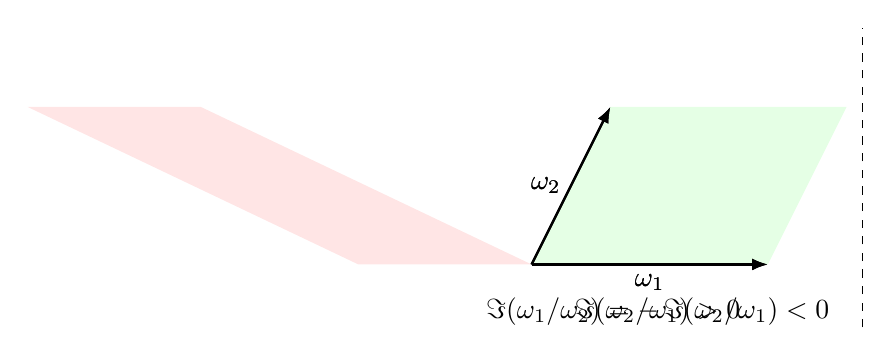
\begin{tikzpicture}[scale=1.0]
			\coordinate (O) at (0,0);
			\coordinate (w1) at (3,0);
			\coordinate (w2) at (1,2);
			
			% First (positive) orientation
			\fill[green!10] (O) -- ($(O)+(w1)$) -- ($(O)+(w1)+(w2)$) -- ($(O)+(w2)$) -- cycle;
			\draw[thick,-{Latex[length=2mm]}] (O) -- (w1) node[midway,below] {$\omega_1$};
			\draw[thick,-{Latex[length=2mm]}] (O) -- (w2) node[midway,left] {$\omega_2$};
			\node at ($(O)+(1.6,-0.6)$) {\(\Im(\omega_2/\omega_1)>0\)};
			
			% Separator
			\draw[dashed] (4.2,-0.8) -- (4.2,3.0);
			
			% Second (swapped) orientation
			\begin{scope}[shift={(5.2,0)}]
				\fill[red!10] (O) -- ($(O)+(w2)$) -- ($(O)+(w2)+(w1)$) -- ($(O)+(w1)$) -- cycle;
				\draw[thick,-{Latex[length=2mm]}] (O) -- (w2) node[midway,left] {$\omega_2$};
				\draw[thick,-{Latex[length=2mm]}] (O) -- (w1) node[midway,below] {$\omega_1$};
				\node at ($(O)+(1.6,-0.6)$) {\(\Im(\omega_1/\omega_2)= -\,\Im(\omega_2/\omega_1)<0\)};
			\end{scope}
		\end{tikzpicture}
	\end{center}
	
	\section*{7. Quick checks and exercises}
	\begin{itemize}
		\item \textbf{Check 1 (Nondegeneracy).} Show \(\Im(\tau)\neq 0\) iff \(\omega_1,\omega_2\) are \(\R\)-independent.
		\item \textbf{Check 2 (Area formula).} Prove Lemma~\ref{lem:area} directly by expanding
		\(\det\begin{psmallmatrix}\Re\omega_1 & \Re\omega_2\\ \Im\omega_1 & \Im\omega_2\end{psmallmatrix}\)
		and comparing with \(|\omega_1|^2\Im(\omega_2/\omega_1)\).
		\item \textbf{Exercise (Modular action).} Verify
		\(\displaystyle \Im\!\left(\frac{a\tau+b}{c\tau+d}\right)=\frac{\Im\tau}{|c\tau+d|^2}\)
		and conclude that \(\Hh\) is stable under \(\mathrm{SL}_2(\Z)\).
		\item \textbf{Exercise (Normalization).} Using scaling, put \(\omega_1=1\). Using orientation,
		arrange \(\Im(\tau)>0\). Explain why this is a canonical choice up to \(\mathrm{SL}_2(\Z)\).
	\end{itemize}
	
	\section*{8. One-sentence summary}
	We require \(\Im(\omega_2/\omega_1)>0\) to ensure the pair \((\omega_1,\omega_2)\) generates a genuine rank-2 lattice (nondegenerate), gives it a consistent orientation (positive signed area), and yields a unique parameter \(\tau\in\Hh\) modulo \(\mathrm{SL}_2(\Z)\), which cleanly parametrizes isomorphism classes of complex tori.
	
\end{document}
